\section{Exploring Bias Mitigation in ChatGPT through Zero-Shot Prompt Learning with ICQ}
\label{sec:mitigatingbiases}
\begin{figure}[th]
\centering
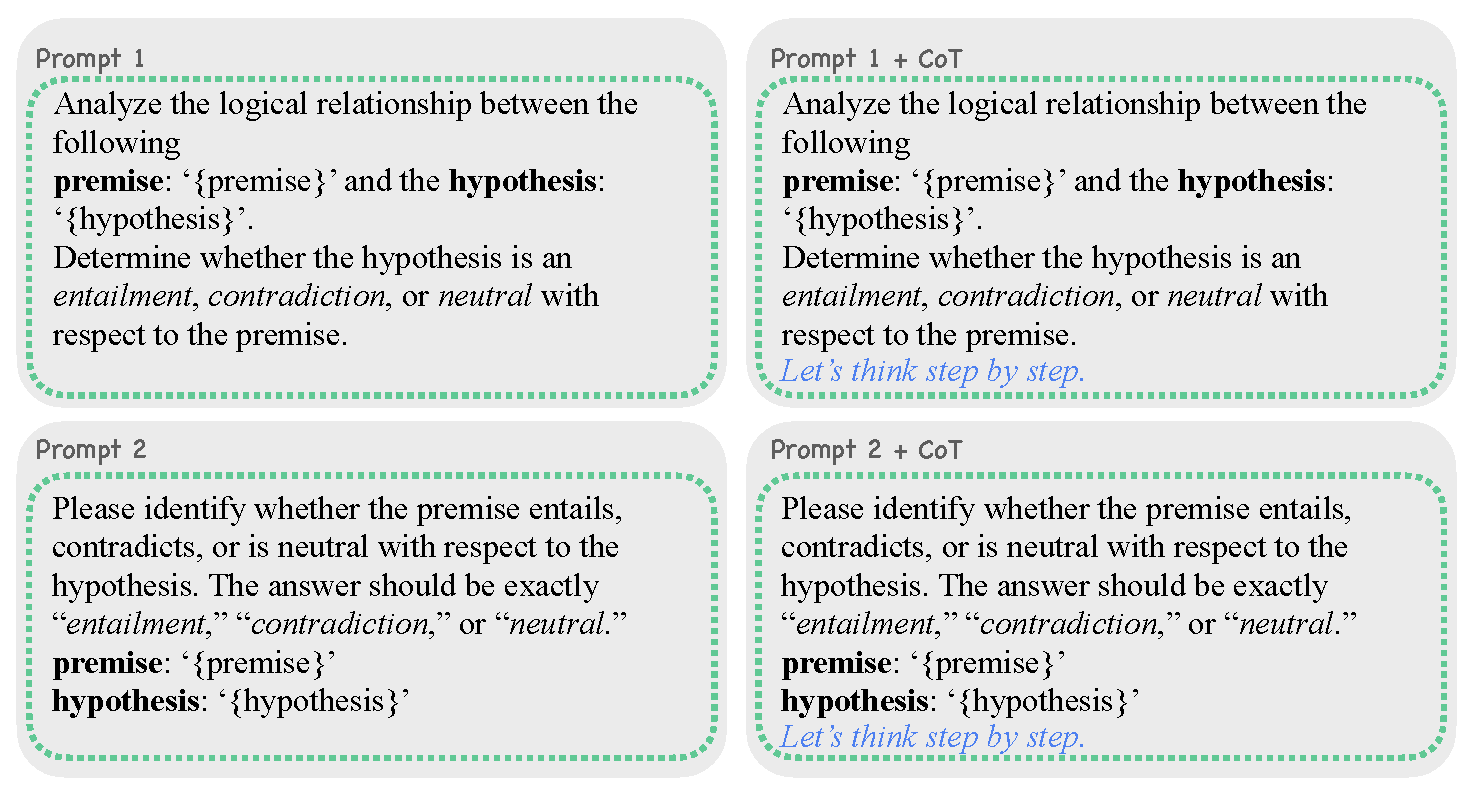
\includegraphics[width=\columnwidth]{picture/prompt.eps}
\caption{Prompts. }
%\KZ{``Possible distributions of the same feature''}}
\label{fig:prompt}
\end{figure}

Recently, ChatGPT, a large language model (LLM) released by OpenAI, has garnered significant interest 
from the NLP community.
ChatGPT, a GPT-x~\footnote{Currently, X is either 3.5 or 4, and in the subsequent experimental process, the ChatGPT we use is based on GPT-3.5.} series model, 
is trained through Reinforcement Learning from Human Feedback (RLHF)~\cite{christiano2017deep} similarly to InstructGPT~\cite{ouyang2022training}.
In this section, we investigate if zero-shot ChatGPT is influenced by bias features, using a case study focused on the word ``no'' in the MNLI dataset.
We aim to compare the effectiveness of different prompts and select the best one for mitigating bias. 

\subsection{Dataset}
\label{sec:chatgptdata}
We selected test instances from the MNLI dataset 
to study the influence of the word ``no'' on ChatGPT's performance. 
The original test set has \textit{Contradiction}: 3240, 
\textit{Entailment}: 3463, and \textit{Neutral}: 3129 instances. 
Instances containing ``no'' are distributed as follows: \textit{Contradiction}:, 
\textit{Entailment}: 38, and \textit{Neutral}: 46.

For the accuracy test, we used all 313 instances i
with ``no'' and an equal number of instances without 
``no'', randomly chosen from the remaining test set. 
This ensures a balanced evaluation of ChatGPT's performance.

For the distribution test, we selected 38 
instances per label containing ``no'', 
resulting in a total of 114 instances. 

\subsection{Prompt Design}
We design four types of prompts in~\figref{fig:prompt}:
The first prompt is proposed by ChatGPT itself. 
We ask, ``What is the best prompt for the MNLI task according to you?''. 
ChatGPT returns prompt 1 for us. 
The second prompt is inspired by previous work~\cite{qin2023chatgpt}.
The third and fourth prompts are created by adding ``Let's think step by step''~\cite{kojima2022large}
to prompt 1 and prompt 2 with the ``chain of thought'' (CoT) thinking, respectively. 
This modification has been shown to significantly improve 
the performance of InstructGPT on reasoning tasks~\cite{ouyang2022training}.

\subsection{ICQ Results}
\label{sec:chatgptacc}
\begin{table}[th]
\centering
\begin{minipage}{0.45\linewidth}
\centering
\scriptsize
\begin{tabular}{c|ccc}
\toprule
\textbf{Prompt} & Acc (``no'') & Acc (w/o ``no'') & $\Delta Acc$ \\ \midrule
P1  & 74.34& 77.32& -2.98   \\ \hline
P2&  75.42& 74.18 & 1.24 \\ \hline
P1 + CoT  & 78.35& 77.28&1.07  \\ \hline
P2 + CoT&  76.67& 76.40&  0.27 \\ \hline
 \bottomrule
\end{tabular}
\caption{Accuracy test results (\%). P1=Prompt 1, P2=Prompt 2.}
\label{tab:accuracy}
\end{minipage}\hfill
\begin{minipage}{0.45\linewidth}
\centering
\scriptsize
\begin{tabular}{c|ccc}
\toprule
\textbf{Prompt} & Entailment & Neutral & Contradiction \\ \midrule
P1&  12&    10&  16\\ \hline
P2 &  13 &    6&  19 \\ \hline
P1 + CoT  & 14& 10&  14 \\ \hline
P2 + CoT & 13& 11&  14\\ \hline
 \bottomrule
\end{tabular}
\caption{Distribution test results.}
\label{tab:distribution}
\end{minipage}
\end{table}

We evaluated the model's accuracy using different prompts on instances 
with and without the word ``no.'' The results are shown in~\tabref{tab:accuracy}. 
P1 demonstrates a negative $\Delta$ Acc, 
indicating difficulty in generalizing when ``no'' is present. 
P2 exhibits a positive $\Delta$ Acc, suggesting better generalization. 
Adding ``CoT'' to both prompts reduces bias risk. 
P1 + CoT shows the most significant improvement in 
Acc (``no''), but P2 + CoT has the smallest absolute 
$\Delta$ Acc, indicating the least sensitivity to ``no'' 
and the lowest bias risk among the tested prompts.

Besides, we analyzed the model's prediction distribution~\tabref{tab:distribution} 
for the different prompts on the stress test set 
containing the word ``no'' with balanced label distribution. 
Distribution test results reveal imbalances in P1 and P2 
prediction distributions, with P1 and P2 leaning towards 
predicting contradictions. Adding ``CoT'' mitigates these imbalances, 
leading to more balanced distributions. 
P2 + CoT presents the most balanced distribution 
among the labels, supporting its lowest bias risk.

In conclusion, 
our case study demonstrates that zero-shot 
ChatGPT can be influenced by bias features, and the 
choice of prompt can have a substantial effect on its performance.
By comparing the effectiveness of different prompts, 
P2 + CoT exhibits the lowest bias risk based on both tests. 
The ``CoT'' strategy is effective in reducing bias risk. 
These findings suggest that ChatGPT's self-recommended prompt 
(P1) may not always be optimal, emphasizing the importance of 
human intervention and continuous exploration to optimize performance and reduce bias risks.
